\chapter{Część praktyczna}
W rozdziale tym przedstawię proces utworzenia aplikacji internetowej oraz mobilnej. Omówię wyzwania oraz problemy, z którymi się spotkałem podczas implementacji. Opiszę też zasadę działania algorytmów potrzebnych do realizacji podstawowych założeń aplikacji mobilnej oraz internetowej. Na koniec przeprowadzę badania i wyciągnę wnioski które skonfrontuje z postawioną tezą.

\section{Przygotowanie}
Aby rozpocząć prace nad utworzeniem aplikacji internetowej i mobilnej potrzebny jest warsztat sprzętowy oraz odpowiedniego oprogramowania zainstalowanego i skonfigurowanego na danym sprzęcie.

\subsection{Sprzęt}
Do wytworzenia aplikacji internetowej oraz mobilnej potrzebny jest komputer. W moim przypadku środowisko programistyczne zainstalowałem i skonfigurowałem na MacBooku Pro z 2011 roku. Do celów badawczych pracy potrzebny mi był smartfon z systemem operacyjnym Android. Wykorzystałem do tego zadania LG Nexus 5. Dodatkowo jeżeli mamy smartfon z systemem Android to nie musimy konfigurować emulatora, co w przypadku mojego komputera mogłoby bardzo ograniczyć zasoby pamięci RAM.

\subsection{Oprogramowanie}
\subsubsection{Git}
Korzystając z nowoczesnych narzędzi wytwarzania oprogramowania naturalnym jest, aby korzystać z systemu kontroli wersji. Osobiście mam doświadczenie z systemem Git. Aby korzystać z takiego systemu potrzebujemy mieć zainstalowane narzędzie klienckie. Ponadto potrzebujemy mieć skonfigurowane repozytoria na odpowiednim serwerze. Ja do tego celu wykorzystałem darmowy plan na platformie Github. Utworzyłem dwa repozytoria, oddzielne dla aplikacji internetowej i aplikacji mobilnej.

\subsubsection{Ruby}
Spośród wielu implementacji oraz narzędzi do zarządzania środowiskiem uruchomieniowym Ruby wybrałem wersję 2.3.3, która na dzień tworzenia projektu była najnowsza. Do zarządzania wersją Ruby wykorzystuję narzędzie rbenv.

\subsubsection{RubyMine}
Mimo że Ruby jest językiem interpretowanym, a zestaw konsolowych narzędzi Ruby on Rails wykorzystuje się w sposób naturalny. Jednak osobiście bardzo lubię korzystać z tego edytora. Podświetlanie składni, refaktoryzacja kodu i integracja z Gitem powodują, że pisanie aplikacji internetowej nie jest toporne i żmudne. Wersja na dzień utworzenia projektu to 2017.1.

\subsubsection{PostgreSQL}
PostgreSQL na środowiska Mac OS można ściągnąć w postaci zwykłej aplikacji systemowej i tak też zrobiłem w swoim projekcie. Aplikacja zasugerowała najnowszą wersję systemu bazy danych i na dzień utworzenia projektu oznaczenie wersji to 9.6.

\subsubsection{Android Studio}
Najprostszym sposobem wytwarzania oprogramowania dla systemów Android jest korzystanie z pakietu Android Studio. Najnowsza wersja na dzień utworzenia projektu to 2.3.2. W ramach instalacji tego środowiska programistycznego zostało zainstalowanych wiele bibliotek. Między innymi SDK Manager, w którym zainstalowałem SDK Platformy o oznaczeniu Android 7.1.1 (Nougat), której poziom API to 25.

\subsubsection{Przeglądarka internetowa}
Gdy mowa o aplikacji internetowej, to nie można zapomnieć o jej kliencie - przeglądarce internetowej. Przy rozwoju aplikacji opartej na Ruby on Rails, nie ma większego znaczenia z jakiej przeglądarki skorzystamy. Osobiście jednak polecam aby na komputerze posiadać przeglądarki kilku firm, ze względu na kompatybilność. Jak się dowiemy w późniejszych rozdziałach, ma to znaczenie przy rozwoju takiej aplikacji internetowej.

\section{Aplikacja internetowa}
Implementację rozpocząłem od importu istniejących danych o lokalizacjach sieci WIFI z różnych serwisów. Potem skupiłem się na prezentacji zaimportowanych danych. Na koniec stworzyłem ścieżkę pod którą można geolokalizować na podstawie podanych adresów MAC i siły sygnałów podanych sieci bezprzewodowych.

\subsection{Struktura danych}
W internecie można znaleźć trzy serwisy, które za darmo udostępniają zrzuty bazy z lokalizacjami bezprzewodowych sieci.

\begin{table}
\caption{Rozmiary i format zrzutów baz danych z informacjami o lokalizacjach sieci bezprzewodowych}
\label{table:wifilocationdatabases}
\begin{tabular}{ |l|l|l|  }
\hline
Adres serwisu & Rozmiar danych & Fromat \\
\hline
\hline
openwifi.su (openwlanmap.org) & 245,7MB & CSV spakowany do tar.bz2 \\
\hline
mylnikov.org & 657 MB & CSV spakowany do zip \\
\hline
radiocells.org (openbmap) & 1.6GB & baza danych sqlite \\
\hline
\end{tabular}
\end{table}

Na podstawie importowanych danych przygotowałem strukturę bazy danych obserwacji. Uwzględniłem też kolumny, które będą potrzebne przy zbieraniu obserwacji z aplikacji mobilnej. Tablica \ref{table:dbscheme}

\begin{table}
\caption{Kolumny i typy przechowywania danych wraz z ich znaczeniem}
\label{table:dbscheme}
\begin{tabular} { |l|l|l|p{6cm}|  }
\hline
Typ & Nazwa & Dodatkowe uwagi & Znaczenie (opcjonalne) \\
\hline
\hline
string   & bssid & null: false & \\
\hline
string   & ssid & & \\
\hline
datetime & observed\_at & & Informacja kiedy dana sieć została zaobserowana \\
\hline
float    & latitude & null: false & Szerokość geograficzna \\
\hline
float    & longitude & null: false & Wysokość geograficzna \\
\hline
datetime & geolocated\_at & & Gdy urządzenie rozróżnia czas ostatniej pozycji GPS od czasu obserwacji sieci bezprzewodowej \\
\hline
string   & source & default: "internal" & Nazwa źródła skąd przyszły dane. Jeżeli import to odpowiednia nazwa serwisu. Jeżeli z aplikacji mobilnej, to odpowiedni identyfikator urządzenia \\
\hline
string   & id\_of\_source & & Identyfikator w ramach pola source - pozwoli na nie importowanie duplikatów lub możliwą aktualizację importowanych danych \\
\hline
json     & raw\_info & & Wszystkie atrybuty jakie były zadeklarowane do obserwacji. Jeżeli byśmy importowali jakieś dane, które nie mają odpowiedniej kolumny w bazie danych, to w przyszłości możemy te dane wyciągnąć z tej kolumny. \\
\hline
datetime & created\_at & & Data i czas utworzenia rekordu (domyślnie dodawane przez Ruby on Rails) \\
\hline
datetime & updated\_at & & Data i czas modyfikacji rekordu (domyślnie dodawane przez Ruby on Rails) \\
\hline
\end{tabular}
\end{table}

Ze względu na prędkość importu zdecydowałem się zdenormalizować obserwacje punktów dostępów. Kolumna BSSID - opisującą adres sprzętowy urządzenia będzie posiadała powtarzające się dane. Dzięki temu mogłem użyć biblioteki activerecord-import. Która pozwala na import danych do bazy danych poprzez bardzo praktyczny interfejs, ale przede wszystkim w sposób bardzo szybki. Dzięki tej decyzji import informacji o lokalizacjach sieci bezprzewodowych dla obszaru Warszawy zajął prawie 6 godzin na moim komputerze.

\subsection{Prezentacja danych na mapie}
Do prezentacji danych jakimi są lokalizacje sieci bezprzewodowych wykorzystałem gotową bibliotekę Leaflet. Wykorzystywanie gotowych elementów interfejsu często przyspiesza pracę nad projektami. Zwłaszcza tak skomplikowanego interfejsu jakim jest mapa. Sama biblioteka implementuje obsługę współrzędnych geograficznych, przybliżania i oddalania oraz prostych znaczków i kształtów geograficznych. Podstawowym elementem jaki musiałem dodać to grafiki mapy - tzw. płytki map (z ang. map tiles). Mój wybór padł na dostawcę darmowych grafik - serwis CartoDB. Udostępniają oni wysokiej jakości, schludne grafiki do wyboru w kilku odcieniach. Na potrzeby tej pracy wybrałem minimalistyczną i ciemną wersję o nazwie dark. Do Leafleta dodałem jeszcze dwa dodatki: jeden odpowiedzialny za pobieranie danych standardem AJAX oraz drugi, który jest odpowiedzialny za klastrowanie dużej ilości znaczników na mapie w grupy.

Dla widoku mapy utworzyłem ścieżkę na serwerze, pod którą można pobrać znaczniki z lokalizacjami sieci bezprzewodowych. Zdecydowałem się na strukturę danych określoną w standardzie GeoJSON ze względu na

%Ze względu na ogrom danych jakimi są zapisane lokalizacje sieci bezprzewodowych, potrzebne jest wykorzystanie mechanizmu AJAX.

\subsection{Algorytm geolokalizacji}
Podstawą algorytmu jest średnia ważona współrzędnych geograficznych pozycji sieci bezprzewodowych o najmocniejszym sygnale, znalezionych na podstawie podanych adresów MAC, a gdzie waga będzie wyliczana na podstawie:

\begin{itemize}
\item daty ostatniej obserwacji
\item podanej siły sygnału
\item nieliniowego współczynnika odchylenia lokalizacji od innych lokalizacji sieci bezprzewodowych - jego zadaniem jest eliminacja lub ograniczenie znaczenia sieci, których lokalizacja w bazie danych może być nieaktualna
\end{itemize}

\section{Aplikacja mobilna}
\subsection{Baza danych}
% denormalizowana
% wykorzystująca ORM ActiveAndroid
\subsection{Mapa}
% trzeba było włączyć CORS

\subsection{Wardriving}
\subsubsection{Standard \_nomap i \_opt\_out}
Google zaproponowało dopisywanie do końca nazwy sieci \_nomap (z ang. nie mapuj) aby ich rozwiązania nie zbierały informacji o lokalizacji danych sieci bezprzewodowych.\cite{GoogleNomap} Dodatkowego zamieszania dorzuciła firma Microsoft gdzie dla swoich rozwiązań zaproponowali \_optout (z ang. wypisz mnie).\cite{MicrosoftOptout}

%\subsubsection{Zbieranie nazw sieci wifi}
%Prawo w stanach zabrania jakieś źródła czy cuś
\subsubsection{Problem z określeniem lokalizacji}
Nie jest możliwym stwierdzenie z jakiego kierunku przyszedł sygnał. Co przy mapowaniu przy użyciu telefonu komórkowego spodowuje umiejscowienie wszystkich sieci wifi na pozycji telefonu. Np. na środku ulicy lub na chodniku.
Ze względu na lokalizację między dwoma punktami klient-serwer.
% widać to świetnie na tej mapie: http://owm.vreeken.net/map/
% zrobić obraze

\begin{figure}[h!]
  \centering
    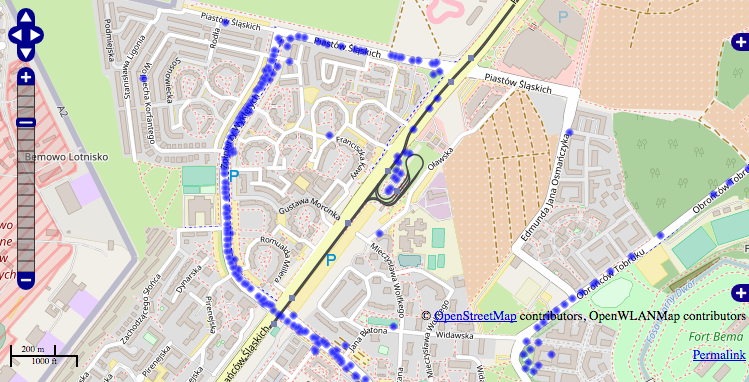
\includegraphics[width=10cm]{images/poor-scan-result}
  \caption{Prezentacja lokalizacji sieci bezprzewodowych na mapie - algorytm primitywny}
  \label{fig:warsaw10kmRadius}
\end{figure}

Rozwiązaniem droższym byłoby użycie kilku urządzeń, najlepiej z antenami kierunkowymi, dzięki czemu moglibyśmy stwierdzić czy stacja bazowa znajduje się po lewej stronie ulicy czy po prawej na podstawie siły sygnału.
Dzięki technologii MIMO można określić z którego kierunku przyszedł sygnał na jednym urządzeniu.


\section{Publikacja projektu}
\subsection{Zakup domeny}
geowifi.science
\subsection{Maszyna wirtualna}
Azure
\subsubsection{Cloudflare}
Konfiguracja
\subsection{Publikacja aplikacji na Google Play Market} %czy jak to sie tam nazywa
